\documentclass{article}
\usepackage[margin=3cm]{geometry}
\usepackage{graphicx}
\usepackage{subcaption}

\newcommand{\supphyperradverify}{1}
\newcommand{\suppcomponorm}{2}
\newcommand{\suppfdr}{3}
\newcommand{\suppannotate}{4}

\newcommand{\suppfighyperrad}{S1}
\newcommand{\suppfighypertol}{S2}
\newcommand{\suppfignbdisp}{S3}
\newcommand{\suppfigfdr}{S4}
\newcommand{\suppfigrealextra}{S5-9}
\newcommand{\suppfignonlinear}{S10}
\newcommand{\suppfigclustersim}{S11}
\newcommand{\suppfigclusterreal}{S12}

\newcommand{\supptabparam}{S1}

\title{Testing for differential abundance in mass cytometry data}
\author{Aaron T. L. Lun, Arianne C. Richard and John C. Marioni}

\usepackage{setspace}
\spacing{1.5}

\begin{document}
\maketitle

\begin{quote}
\textbf{Abstract:} Mass cytometry is a recently developed technique that allows researchers to simultaneously quantify the expression of many protein markers in each of millions of cells. 
One key challenge is to identify ``differentially abundant'' subpopulations, where the fraction of cells from a given subpopulation differs between biological conditions. 
Here, we present a novel computational strategy for detecting differentially abundant subpopulations in a statistically rigorous manner. 
Our approach quantifies the abundance of subpopulations across the high-dimensional marker space by assigning cells into hyperspheres, thereby avoiding uncertainties introduced by clustering of the data. 
Within each hypersphere, we test for significant changes in the proportion of cells from each biological condition, before using a spatial false discovery rate to correct for multiple testing across the high-dimensional space. 
We demonstrate the utility of our approach by applying it to simulated data, where it outperforms a simple clustering-based approach, as well as a real dataset characterising the reprogramming of murine embryonic fibroblasts to induced pluripotent stem cells, where it detects both known and novel subpopulations.
\end{quote}

\section{Introduction}
Mass cytometry is a recently developed technique that allows researchers to simultaneously characterise the expression of many ($>30$) protein markers in each of millions of cells \cite{ornatsky2008study}.
Briefly, antibodies specific to markers of interest are conjugated to heavy metal isotopes and used to stain a population of cells.
The suspension of stained cells is passed through a nebulizer and single-cell droplets are vaporized to release and ionize the metals.
Finally, the quantity of metal ions produced from each cell is measured by time-of-flight mass spectrometry.
The resolution of mass spectrometry on purified isotopes avoids problems with spectral overlap that are frequently encountered in conventional flow cytometry with fluorescent markers.
This means that more markers can be quantified for each cell, improving resolution of distinct subpopulations and increasing the potential to obtain novel biological insights.

The ability of mass cytometry to assay more markers leads to a concomitant increase in the dimensionality of the data.
This complicates the data analysis as manual gating and visual examination of biaxial plots are no longer feasible when many possible marker combinations have to be considered.
Instead, bespoke computational methods are required to extract meaningful biological information from mass cytometry data. 
To this end, a number of software tools have been developed, including SPADE \cite{qiu2011extracting} and X-shift \cite{samusik2016automated}.
These methods have focused on clustering cells into biologically relevant subpopulations based on the ``intensity'' of each marker (i.e., the signal of the corresponding isotope in the mass spectrum) and quantifying the abundance of each subpopulation in the total cell pool.
This exploits the availability of a large number of markers in mass cytometry data to effectively distinguish subpopulations.

Another analytical approach is to identify empirical subpopulations that change in abundance between conditions.
For example, immune compartments are enriched or depleted following drug treatment or pathogen challenge, and the composition of cell types changes during development and ageing.
Detection of these differentially abundant (DA) subpopulations is useful as it can provide insights into the cause or effect of the biological differences between conditions.
From a statistical perspective, it is also more straightforward to compare abundances between samples for the same subpopulation than comparing abundances between subpopulations.
In the former setting, any subpopulation-specific biases (e.g., due to antibody-specific effects) are expected to cancel out and can be ignored, thus simplifying the downstream analysis.

Testing for DA subpopulations is a routine step in flow cytometry studies \cite{saeys2016computational,mittag2011recent}, but few methods are available to perform this analysis on mass cytometry data.
Of the methods that do exist, the typical strategy involves clustering cells from all samples into empirical subpopulations before checking each cluster for differential abundance \cite{anchang2016visualization,bruggner2014automated}.
While intuitive, this approach is sensitive to the parametrization of the initial clustering step.
Uncertainty will be introduced into the cluster definitions when the data are noisy or the cells are not clearly separated \cite{suzuki2006pvclust,kerr2001bootstrapping}.
This is problematic if a DA subpopulation is incorrectly placed into the same cluster as a non-DA subpopulation -- hence, any change in the former will be masked by the latter.
Conversely, relying only on well-separated clusters will result in loss of power to resolve subpopulations that differ only subtly.
Furthermore, cluster formation also depends upon the choice of algorithm \cite{datta2003comparisons,wiwie2015comparing}, which can make it difficult to determine the reliability of the clusters.

% - SPADE uses downsampling to avoid loss of rare things, but it still caps the maximum number of clusters; if there's more than 200 subpops, you're in trouble.
% - Merged clusters would still also see a change in marker intensity, so theoretically still could be detected; however, this would be a lot weaker, so power would be reduced.
% - The Anchang paper is more descriptive with regards to abundances. CITRUS will test significance of correlations between abundance and group, so I'll let it go.

Here, we present a DA analysis pipeline for mass cytometry data that does not rely on an initial clustering step.
Cells from multiple samples are assigned to high-dimensional subspaces, and counts for each subspace are tested for significant differences between conditions.
To correct for multiple testing, we describe the concept of the spatial false discovery rate and present a method to control it.
Significant subspaces are then visualized in lower dimensions for manual annotation, allowing domain expertise to be incorporated during the interpretation of the results.
In this manner, DA subpopulations can be identified while avoiding the uncertainties and errors associated with clustering.
We demonstrate the use of our pipeline on public data \cite{zunder2015continuous}, where we recover both known and previously uncharacterised subpopulations that change in abundance across a reprogramming time course.

\section{Overview of the differential abundance pipeline}
Our analysis pipeline for detecting differential abundance can be split into three parts (Figure~\ref{fig:overview}). 
Firstly, we count cells into hyperspheres in the multi-dimensional marker space.
Each hypersphere contains a subset of cells and is defined by a combination of marker intensities.
We perform this counting for each sample in each biological condition, such that each hypersphere is associated with a set of cell counts.
Secondly, we use the count data for each hypersphere to test for significant differences in cell abundance between conditions.
Finally, we use the hypersphere $p$-values to control the false discovery rate (FDR) across the multi-dimensional space, i.e., the spatial FDR.
Dimensionality reduction is then performed on the significant hyperspheres to visualize DA subpopulations.

\begin{figure}[bt]
\begin{center}
    \includegraphics[width=\textwidth]{pics/pipeline.pdf}
\end{center}
\caption{Diagram of the differential abundance pipeline.
    (A) Cells from samples 1 (pink) or 2 (light blue) are distributed across the multi-dimensional marker space (two markers shown here for simplicity).
    Hyperspheres (yellow) centred on selected cells are constructed, and the number of cells from each sample inside each hypersphere is counted.
    (B) Counts for each hypersphere are tested for significant differences between samples.
    This yields a $p$-value representing the evidence against the null hypothesis of no differences.
    (C) Multiple testing correction of hypersphere $p$-values is performed by controlling the spatial FDR.
    Positions of significant hyperspheres are visualized by dimensionality reduction (e.g., PCA), where the expected proportion of false positives is kept below some threshold.
}
\label{fig:overview}
\end{figure}


We demonstrate the application of our pipeline to data from a study of mouse embryonic fibroblast (MEF) reprogramming \cite{zunder2015continuous}.
In this study, primary and secondary MEFs were used for reprogramming.
Primary MEFs expressing green fluorscent protein (GFP) from the endogenous Oct4 locus (Oct4-GFP) were transduced with lentiviruses expressing a doxycycline-inducible suite of reprogramming factors.
Secondary MEFs expressing either GFP or a neomycin resistance gene (Neo) from the endogenous Nanog locus (Nanog-GFP or Nanog-Neo, respectively) already harboured doxycycline-inducible reprogramming transgenes.
For each MEF reprogramming system, a time course was constructed by taking samples at days 0-30 after doxycycline-induced transgene expression.
Samples in the same time course were barcoded, stained with metal-conjugated antibodies and profiled by mass cytometry.
The aim of our re-analysis of this data is to detect subpopulations that change in abundance over time.

\section{Summarizing the cell distribution with hyperspheres}
Consider a mass cytometry data set with $S$ samples and $M$ markers.
We assume that appropriate transformations (e.g., biexponential) have been applied to the marker intensities.
We also assume that normalization of marker intensities between samples, if necessary, has already been performed.
In the MEF reprogramming data set, the data was collected by multiplexing of barcoded samples \cite{zunder2015palladium}, so no normalization of intensities is required between samples.
Each cell in each sample defines a point in the $M$-dimensional space, with coordinates defined by its transformed (and normalized) intensities.

We quantify the abundance of cells across the space by considering $M$-dimensional hyperspheres.
Each hypersphere defines a subspace that is centred at a distinct combination of marker intensities.
We count the number of cells from each sample that lie inside each hypersphere, yielding $S$ counts per hypersphere.
(While each subspace contains a subset of cells in the population, this should not be confused with a cell subpopulation.
The latter refers to a biologically meaningful or functional subset, while the former is simply an analytical construct used for cell counting.)
For each marker, we also compute the median intensity for all cells in each hypersphere.
This provides a median-based position for the hypersphere, representing the central location of the subspace around which most of the cells in the hypersphere originated.
The median position is more appropriate than the hypersphere centre when the cells counted into the hypersphere are not symmetrically distributed around the centre.

%We then test for differences in the counts between samples, to determine whether the cell abundance in that subspace changes between biological conditions.
%Repeating this process for all hyperspheres will identify differentially abundant subspaces.

The radius $r$ of each hypersphere is a pre-defined value that must be large enough to obtain large counts, yet small enough to avoid counting cells from adjacent subspaces.
We set $r=0.5\sqrt{M}$ to offset the increasing sparsity of the data as the number of dimensions increases.
The 0.5 scaling factor represents the acceptable variability of the intensities for each marker.
Specifically, transformed intensities lie on the $\log_{10}$-scale, so a value of 0.5 ensures that cells with a 10-fold difference in marker expression are routinely counted into the same hypersphere.
This strategy is motivated by the fact that technical or biological variability often results in an order of magnitude difference in observed expression within the same functional subpopulation \cite{ornatsky2008study,zunder2015continuous,zunder2015palladium}.
We verify this choice of $r$ in the MEF reprogramming data where the distance between neighbouring cells increases as a square-root function of $M$ (Figure~\suppfighyperrad{}).
Setting the scaling factor to 0.5 also ensures that counts are large enough for further analysis (Figure~\suppfighypertol{}).
See Section~\supphyperradverify{} and Table~\supptabparam{} of the Supplementary Materials for more details.

Each hypersphere is also centred at a point defined by an existing cell.
This is necessary because there are an infinite number of hyperspheres in the $M$-dimesional space.
Centering on existing cells ensures that only non-empty hyperspheres are considered.
In practice, we further reduce computational work by only constructing hyperspheres at every (randomly chosen) 10\textsuperscript{th} cell.
This avoids redundant work in high-density subspaces where many of the resulting hyperspheres would be near-identical in terms of their positions and cell counts.
Note that many adjacent hyperspheres will be overlapping -- this has some implications for FDR control which will be discussed in more detail later.

\section{Testing for differential abundance in each hypersphere}
Once the counts are obtained, each hypersphere can be tested for differential abundance between conditions.
The null hypothesis is that there is no change in the average counts between conditions within each hypersphere.
Testing can be performed with standard methods for analyzing count data, e.g., negative binomial generalized linear models (NB GLMs).
The NB model is useful as it explicitly accounts for the discrete nature of counts, while also modelling overdispersion due to biological variability between replicate samples (Figure~\suppfignbdisp{}).
GLMs can also accommodate complex experimental designs involving multiple factors and covariates.
For example, each time course in the MEF reprogramming data set can be modelled by fitting a time-dependent trend to the counts for each hypersphere.

We can implement NB GLMs using standard methods in statistical software like R, or through existing R packages like edgeR \cite{robinson2010edgeR} or DESeq2 \cite{love2014moderated}.
The latter were originally designed for analyzing read count data from RNA sequencing experiments.
However, the same mathematical framework can be applied to cell counts in mass cytometry data.
In particular, information can be shared across hyperspheres via empirical Bayes \cite{mccarthy2012differential, lund2012detecting}.
This improves estimation of the dispersion parameter in the presence of limited replicates, thus increasing the reliability and power of downstream inferences.

We also normalize the counts for each hypersphere based on the total number of cells in each sample.
This accounts for differences in the input quantities of cells between different samples.
Specifically, we define the GLM offsets as the log-transformed total number of cells in each sample.
This is conceptually equivalent to analyzing the \textit{proportion} of cells in each sample that are located inside each hypersphere.
Note that this approach does not protect against composition effects -- see Section~\suppcomponorm{} of the Supplementary Materials for some strategies to deal with these effects, if they are of concern.

We tested the performance of edgeR using simulations constructed from the MEF reprogramming study.
The observed type I error rate was close to or below the specified threshold for all tested data sets, simulation schemes and threshold values (Figure~\ref{fig:alpha}).
To evaluate power, we compared edgeR to the Mann-Whitney test that is often used to detect differential proportions in flow cytometry data \cite{watson1992significance}.
The Mann-Whitney test routinely yields larger $p$-values than edgeR (Figure~\ref{fig:power}), due to the loss of power from using ranks with small sample sizes.
These results indicate that edgeR is both specific and sensitive, and thus is appropriate for detecting differential abundance in mass cytometry data.

\begin{figure}[bt]
\begin{subfigure}[b]{0.48\textwidth}
    \includegraphics[width=\textwidth]{../simulations/plot_alpha.pdf}
\caption{}
\label{fig:alpha}
\end{subfigure}
\begin{subfigure}[b]{0.48\textwidth}
    \includegraphics[width=\textwidth]{../simulations/plot_power.pdf}
\caption{}
\label{fig:power}
\end{subfigure}
\caption{
Performance of edgeR for detecting DA hyperspheres, using simulations based on the MEF reprogramming time courses.
(\subref{fig:alpha}) Observed type I error rates with edgeR for each time course, using Poisson or overdispersed sampling of cells.
Bar heights represent the mean of 10 simulation iterations, with error bars representing standard errors.
The red lines denote the specified thresholds of 0.01 (left) or 0.05 (right).
(\subref{fig:power}) Log$_{10}$-ratios of the $p$-values computed by edgeR against those from the Mann-Whitney (MW) test, plotted against log$_{2}$-fold changes.
Simulations were performed using overdispersed sampling for the Oct4-GFP time course, and each hypersphere was tested for differential abundance.
Coloured points represent hyperspheres with absolute log-fold changes greater than two and $p$-values that are smaller in edgeR compared to the MW test (orange) or vice versa (blue).
The number of such hyperspheres is also reported.
The size of each point is determined by the edgeR $p$-value.
}
\label{fig:testtest}
\end{figure}

\section{Controlling the spatial false discovery rate}
We define the ``spatial FDR'' as the false discovery rate (FDR) across the $M$-dimensional space.
To illustrate, split the $M$-dimensional space into arbitrarily small non-overlapping partitions of similar volume, e.g., pixels for 2D space or voxels for 3D space.
The aim is to control the FDR across the partitions that contain differential cell abundances.
This error rate is relevant to a validation strategy that performs follow-up studies on each partition. 
(Obviously, in practice, not every partition would be checked due to redundancy between adjacent partitions.
However, the FDR across a random subset of partitions should be similar to that across all partitions, so the spatial FDR is still relevant.)

We stress that the partitions described above are purely conceptual.
The actual tests were performed on the hyperspheres, as the counts for each partition would be too small.
To relate the former to the latter, we assign each DA hypersphere to a partition.
This is done by identifying the partition containing the median-based position of the hypersphere.
The outcome of the differential tests for the hypersphere is used as a proxy for the outcome of its assigned partition (Figure~\ref{fig:fdrdemo}).
If multiple hyperspheres are assigned to a partition, one is randomly sampled to be a representative of that partition.
The FDR across representative hyperspheres is treated as the practical value of the spatial FDR.  

\begin{figure}[bt]
    \begin{center}
        \includegraphics[width=\textwidth]{pics/spatial_fdr.pdf}
    \end{center}
    \caption{
        Assignment of hyperspheres to hypothetical partitions.
        Each point represents the median-based position of a hypersphere in a data set with two markers, coloured based on its test outcome
        (hyperspheres with no significant differences are marked in white, while false positives are in grey).
        Each hypersphere is assigned to a partition, and the test outcome of each partition is defined as that of its hyperspheres.
        For simplicity, all hyperspheres in a partition have the same outcome here.
        The aim is to then control the spatial FDR across partitions, rather than the FDR across hyperspheres.
    }
    \label{fig:fdrdemo}
\end{figure}

We control this FDR by calculating, for each hypersphere, the local density of neighbouring hyperspheres.
This is done by applying a kernel density estimator to the median-based positions of all tested hyperspheres.
We define the weight of each hypersphere as the reciprocal of its local density.
This presumes that the probability of sampling a representative hypersphere from a partition is inversely proportional to the density of assigned hyperspheres in that partition.
For small partitions of similar size, the local density of each hypersphere approximates the density of the partition to which it was assigned.
Thus, the weight of each hypersphere represents the expected frequency of sampling it as a representative (scaled by some constant).
The Benjamini-Hochberg (BH) method is applied to the hypersphere $p$-values with these weights -- see Section~\suppfdr{} of the Supplementary Materials for more details.
In this manner, the FDR across the expected set of representative hyperspheres can be controlled.

We performed simuations based on the MEF reprogramming data to test the use of density-based weights.
We found that the weighting method was able to control the spatial FDR close to or below the specified threshold (Figure~\ref{fig:fdr}).
In comparison, na\"ive application of the BH method (i.e., without weighting) failed to control the spatial FDR.
This is because the na\"ive approach controls the FDR across hyperspheres rather than partitions.
Recall that hyperspheres are centred at existing cells, so any variability in the density of cells across the $M$-dimensional space will lead to variability in the density of hyperspheres across partitions.
As a result, the FDR across hyperspheres may be quite different from that across partitions, such that control of the former will not guarantee control of the latter.
(Differences in spatial density of hypersheres is the main problem with overlapping hyperspheres, as alluded to earlier.
For example, if we consider the differential hyperspheres in Figure~\ref{fig:fdrdemo}, the na\"ive FDR across hyperspheres would be 5\% while the spatial FDR across partitions would be 25\%.)
%Overlapping hyperspheres also introduce dependencies between tests, with which the BH method is not guaranteed to work 
%-- however, in practice, the method is robust to dependencies, so this is less of a concern.)
The weighting approach performs better as it explicitly aims to control the FDR across partitions.
%Some liberalness is still present as the spatial FDR is controlled in $M$-dimensional space while being measured in 2D space after dimensionality reduction.
%Nonetheless, it is clear that density weighting improves the accuracy of spatial FDR control.

\begin{figure}[bt]
\begin{center}
\includegraphics[width=0.9\textwidth]{../simulations/plot_FDR.pdf}
\end{center}
\caption{
    Control of the spatial FDR using the na\"ive and weighted BH methods, in simulations based on the MEF reprogramming time courses.
    The observed spatial FDR was calculated in two-dimensional space using pixel widths of 0.5 to 2.
    Bar heights represent the mean of 50 simulation iterations, and the error bars represent standard errors.
    The red line denotes the nominal threshold of 5\%.
}
\label{fig:fdr}
\end{figure}

\section{Interpreting the results of the DA analysis}
After controlling the spatial FDR, dimensionality reduction is performed on the putative DA hyperspheres.
This yields a low-dimensional representation of the subspaces with altered abundances for plotting.
The plot is annotated based on examination of the marker intensities, incorporating domain expertise on the relationships between specific markers and cell types.
In this manner, biologically relevant subpopulations can be identified from the DA hyperspheres.
(A similar step of manual annotation is involved in interpreting the results of other pipelines, e.g., SPADE \cite{anchang2016visualization}.
This is largely unavoidable as it is difficult to incorporate complex biological knowledge into a computational algorithm.)
Our strategy of testing for differences before defining subpopulations ensures that uncertainty in clustering or annotation does not compromise the computed DA statistics.
It also simplifies the interpretation of the results, as only the subset of DA hyperspheres needs to be visualized and annotated.

We applied our pipeline to detect DA subpopulations in each time course of the MEF reprogramming study.
For each time course, cells from all samples were counted into hyperspheres.
Each hypersphere was tested for differential abundance over time using edgeR.
Putative differential hyperspheres were defined as those detected at a spatial FDR of 5\%.
In this manner, we detected 7416 differential hyperspheres in the Oct4-GFP time course, 5947 in the Nanog-GFP time course, and 21545 in the Nanog-Neo time course.
We then applied $t$-SNE \cite{van2008visualizing} on the positions of detected hyperspheres to obtain a 2D plot of differential subspaces (Figure~\ref{fig:oct4}).
For data sets with many differential subspaces, we prefer $t$-SNE to PCA as the former provides cleaner separation of the underlying subpopulations.
Here, we focus on the Oct4-GFP time course for brevity (see Figures~\suppfigrealextra{} for all time courses).

\begin{figure}[p]
    \begin{center}
    \includegraphics[width=0.8\textwidth]{../realdata/livefire/pics/Figure4.png}
\end{center}
    \caption{
        Differentially abundant subpopulations in the Oct4-GFP time course, detected at a spatial FDR of 5\%.
        (A) A $t$-SNE plot of the median positions of DA hyperspheres. 
        Each point represents a hypersphere and is coloured according to its log-fold change in abundance over time.
        Grey points represent hyperspheres with significant but non-linear changes in abundance.
        Subpopulations were annotated based on results in Zunder \emph{et al.} \cite{zunder2015continuous}, with additional distinguishing features for each subpopulation noted in parentheses.
        OSKM: reprogramming factors (Oct4, Sox2, Klf4, c-Myc), NE: non-expressing, MET: mesenchymal-epithelial transition, SC4: partially reprogrammed cell line, ESC: embryonic stem cells, mixed 4F: mixed stoichiometry of the OSKM factors.
        (B) The same plots coloured by the median intensity of selected markers in each hypersphere.
        The colour range for each marker was bounded at the 1\textsuperscript{st} and 99\textsuperscript{th} percentiles of the intensities across all cells.
    }

    \label{fig:oct4}
\end{figure}

We annotated the differential hyperspheres in Figure~\ref{fig:oct4} based on the subpopulations described in the original analysis by Zunder \emph{et al.} \cite{zunder2015continuous}.
(See Section~\suppannotate{} of the Supplementary Materials for details.)
We were able to identify most of the subpopulations as DA, including MEFs with and without overexpression of the reprogramming factors; 
    the ``mixed 4F'' population expressing a mixed stoichiometry of these factors; 
    cells undergoing mesenchymal-to-epithelial transition; 
    and a population similar to the partially reprogrammed SC4 cell line.
We recovered DA subpopulations corresponding to three reprogramming end points, consisting of embryonic stem cell (ESC)-like cells, mesendoderm-like Lin28\textsuperscript{high} cells, and Thy1\textsuperscript{high}mEF-SK4\textsuperscript{high} cells that likely failed to reprogram and instead reverted to a MEF-like phenotype.
In particular, the abundance of MEFs dropped over time while the abundance of ESC-like cells increased, consistent with the effects of reprogramming.
We resolved many of these populations into two subsets based on cell cycle status, as defined by IdU incorporation.
We also identified some distinct DA subpopulations that were not clearly characterised in the original analysis.
Specifically, we observed an increase in potentially apoptotic cells with cleaved Caspase-3;
    a non-linear change in abundance of a subpopulation of SC4-like cells with phosphorylated STAT3, AMPK and PLK1 (Figure~\suppfignonlinear{});
    and a decrease in abundance of a subpopulation of cells simultaneously expressing high levels of the MEF marker Thy1 along with the reprogramming factors Sox2 and Oct4.

We also examined changes in abundance at critical junctures in the time course.
Figure~\ref{fig:importanttime} visualizes the effect of doxycycline-induced transgene expression and doxycycline withdrawal.
In the former, the MEFs decrease in abundance while the mixed 4F population begins to increase, consistent with induction of some of the reprogramming factors.
Upon withdrawal, the mixed 4F and SC4-like subpopulations decrease as cells start to progress towards one of the reprogramming endpoints.
These results indicate that our analysis pipline is capable of recovering known biology, as well as providing greater resolution to identify subtle changes in abundance of previously uncharacterised subpopulations.

\begin{figure}[bt]
    \begin{center}
        \includegraphics[height=2.7in]{../realdata/livefire/pics/Cytobank_43324_4FI_induction.png}
        \includegraphics[height=2.7in]{../realdata/livefire/pics/Cytobank_43324_4FI_withdrawal.png}
        \includegraphics[height=2.7in]{../realdata/livefire/pics/extra_bar.png}
    \end{center}
    \caption{
        Changes in cell abundance after transgene induction with doxycycline (left) or after doxycyline withdrawal (right) in the Oct4-GFP time course.
        Each point in the $t$-SNE plot represents a differential hypersphere, coloured based on the log-fold change during induction (day 0 to 1) or withdrawal (day 16 to 17).
        A prior of 3 was added to each count to stabilize the log-fold changes.
    }
    \label{fig:importanttime}
\end{figure}

\section{Comparing to a cluster-based approach}
As mentioned earlier, existing methods for analyzing mass cytometry data involve an initial clustering step.
We consider an intuitive extension of this approach whereby the counts for each cluster are tested for differential abundance between conditions.
(We note that the existing methods do not explicitly perform DA analyses.
Anchang \textit{et al.} perform an informal and mostly descriptive comparison between samples \cite{anchang2016visualization} while Bruggner \textit{et al.} focus on feature selection within each cluster \cite{bruggner2014automated}.
As such, we do not test these methods directly, but instead use a custom implementation of a cluster-based analysis.)

We tested the performance of the cluster-based approach on some simulated data.
We observe a loss of power to detect DA subpopulations that are part of a continuum (Figure~\suppfigclustersim{}).
Clusters cannot be unambiguously defined in this scenario, such that a cluster corresponding to a DA subpopulation will also include many cells from adjacent non-DA subpopulations.
This is likely to be problematic in situations where subpopulations are not clearly separated.
Examples include gating strategies commonly used in immunophenotyping to characterise T and B cell subsets \cite{finak2016standardizing}, as well as protocols for isolation of haematopoietic stem cell and progenitor populations \cite{wilson2015combined}.
Counting into hyperspheres is more robust as each subspace in the continuum will be tested for differential abundance.

Applying the cluster-based DA analysis to the Oct4-GFP time course data recovers many of the major subpopulations (Figure~\suppfigclusterreal{}).
However, it fails to detect several others, e.g., parts of the SC4-like subpopulation and Nanog\textsuperscript{high} trajectory as well as some cells undergoing mesenchymal-epithelial transition.
Many of the subpopulations in this data set form a continuous trajectory over time \cite{zunder2015continuous}, so suboptimal cluster formation is not unexpected.
This result suggests that the use of hyperspheres does provide some benefits for detecting subtle changes in abundance within complex subpopulations that are difficult to cluster.
It also simplifies the analysis by avoiding the issue of cluster parametrization -- for example, choosing an appropriate number of clusters is not a straightforward process.

\section{Discussion}
In this article, we present a computational pipeline for detecting DA subpopulations from mass cytometry data.
Unlike existing methods, our pipeline performs the differential testing without requiring an initial clustering step and prior to explicitly defining subpopulations.
This reduces the impact of clustering uncertainty or definition errors on the statistical analysis.
We demonstrate the applicability of our method on a public data set where it detects known and uncharacterised DA subpopulations across a reprogramming time course.
This is done in a statistically rigorous manner that accounts for experimental variability in the abundances and controls the spatial FDR to reduce detection of spurious differences.
The use of GLMs also allows the pipeline to accommodate complex experimental designs, including those with multiple conditions, blocking factors or varying levels of replication.

%Some markers are more relevant than others for defining subpopulations, e.g., IdU is less useful when all subpopulations have a subset of cycling cells.
%Similarly, the variability of intensities for cells from the same functional subpopulation can differ between markers, such that the importance of changes in intensity will also differ.
%For example, in T cell populations, CD4 expression is typically bimodal with tight peaks of high or low intensity, while CD25 expression varies more continuously.

%Errors in classification may also cause problems in the DA analysis.
%If cells with a continuum of marker intensities are classified as a single subpopulation, any internal changes in abundance will be masked.
%Conversely, if cells are under-clustered, interpretation is complicated as many redundant subpopulations are reported with only minor differences in marker intensities.
%From a statistical perspective, these errors are difficult to control as the null hypothesis is not obvious when clustering cells into subpopulations.
%Many assumptions would probably be needed to construct a ``random'' subpopulation for hypothesis testing.
%Care is also required to ensure that a subpopulation is defined consistently across samples, otherwise spurious differences in abundance may be observed across conditions.

Our analytical pipeline offers several advantages over the original analysis of Zunder \emph{et al.} \cite{zunder2015continuous}.
The latter is mainly descriptive, whereas the error-controlling procedures in our analysis provide a greater degree of confidence as to whether the detected changes in abundance are real.
Figure~\ref{fig:oct4} also uses both visual dimensions to separate subpopulations, while the original analysis reserves one dimension for time.
Thus, our approach displays the results in a manner that enhances resolution of distinct subpopulations.
While this comes at the cost of temporal resolution, the pipeline is modular so alternative visualization schemes can be easily applied (on the significant hyperspheres, or the cells contained within them) to focus on particular aspects of the data.
For example, methods like SPADE can be applied to organize the detected DA hyperspheres into a tree for visualization of lineages.

A complementary approach to differential analyses is to detect differential marker expression within the same subpopulation.
Given a (manually or automatically defined) subpopulation, the average intensity of a particular marker can be compared between conditions \cite{anchang2016visualization,behbehani2015mass}.
This detects changes in the expression of activation or signalling markers within a subpopulation.
Our pipeline is different in that it tests for changes in the abundance of cells, rather than their marker intensities.
However, these two types of differential events are closely related.
Consider a marker $X$ in subpopulation $Y$ that increases in expression between two conditions. 
In our analysis, this will manifest as the appearance of new subpopulation $Y'$, separated from $Y$ in the high-dimensional space by an increase in the intensity of $X$.
This new subpopulation will then be detected as DA between conditions.
Thus, changes in intensity can be interpreted as changes in abundance for detection with a DA analysis pipeline.

As mass cytometry becomes more accessible, large-scale experiments containing many conditions and replicates are likely to become increasingly routine.
We anticipate that our DA analysis pipeline will be useful for researchers planning to perform comparative studies with such data sets.

% Talk about GLM LASSO here, don't spend too much time on it.

\section{Methods}

\subsection{Data preparation}
We obtained de-barcoded flow cytometry standard (FCS) files for each time course from Cytobank \cite{kotecha2010web} (accession number 43324).
We applied the logicle transformation \cite{parks2006new} to the marker intensities in each sample.
The transformation parameters were estimated with the estimateLogicle function from the flowCore package \cite{hahne2009flowcore}, using pooled cells from all samples in each time course.
(This avoids spurious differences from sample-specific transformation.)
We gated out cell events with low intensities for the two DNA markers (Iridium-191 and 193), where the threshold was defined as three median absolute deviations below the median intensity for the pooled cells.
We saved the transformed and gated intensities into new FCS files for processing with our pipeline.
Only the intensities for relevant markers (i.e., no DNA, barcodes) were used for further analysis.
Note that normalization of marker intensities between samples is not required for this data set because the samples in each time course were barcoded and pooled for antibody staining and mass cytometry.
Thus, any technical biases will be present in all samples and will cancel out when samples are compared in the DA analysis.

\subsection{Statistical methods for testing differences}
To compute $p$-values, we used the quasi-likelihood (QL) methods in edgeR \cite{lund2012detecting}.
First, we filtered out hyperspheres with an average count below 5.
This improves efficiency by removing tests without enough information to reject the null hypothesis \cite{bourgon2010independent}.
For the remaining hyperspheres, we fitted a mean-dependent trend to the NB dispersion estimates \cite{mccarthy2012differential}.
We fitted a NB GLM to the counts for each hypersphere, using the trended dispersion for each hypersphere and the log-transformed total number of cells as the offset for each sample.
We estimated the QL dispersion from the GLM deviance, and stabilized the estimates by empirical Bayes shrinkage towards a second mean-dependent trend.
Finally, we used the QL F-test with a specified contrast to compute a $p$-value for each hypersphere.

For the simulations, we used a design matrix with a one-way layout to fit each GLM.
Contrasts were performed to test for differences between groups.
For the time course analyses, we used a design matrix constructed from B-spline basis matrix with a time covariate and 3 degrees of freedom.
This allows modelling of time-dependent trends.
Contrasts were performed to test that all spline coefficients were equal to zero.
This represents a null hypothesis that time has no effect on abundance.

We also used the Mann-Whitney test on the simulated data.
For each hypersphere, each count was converted into a proportion of the total number of cells in the corresponding sample.
The Mann-Whitney test was applied on these proportions to test for significant differences between groups.

\subsection{Simulations for assessing type I error control}
We used simulations to determine which testing frameworks were able to control the type I error rate for differential abundance analyses.
For each MEF time course, we pooled cells from all samples in the data set.
We generated new samples by randomly sampling cells from the pool, where each new sample contained the same number of cells as one of the original samples.
We separated the new samples into two groups, counted cells into hyperspheres and tested for differential abundance between groups using edgeR or the Mann-Whitney test.
As all cells were sampled from the same pool, the null hypothesis of constant abundance should be true for each hypersphere.
Thus, the $p$-values computed by each framework should be uniformly distributed.
We calculated the observed type I error rate as the proportion of $p$-values below a specified threshold $\alpha$.
Values of $\alpha=0.01$ and 0.05 were tested.

We used two sampling schemes for this simulation.
The first scheme involved sampling with replacement from the pool, where the probability of sampling each cell was the same.
This is the simplest approach but assumes that only sampling noise contributes to variability between replicates.
In practice, additional biological variability will be present, due to differences in the composition of cell populations extracted from replicate animals or cultures.
To represent this, each cell $j$ in the pool was assigned a probability weight $R_{js}$ for sample $s$.
($R_{js}$ was sampled from a Gamma distribution with shape and rate set to 0.01.
These parameters were chosen to yield NB dispersions of 0.5-1.5 per hypersphere, comparable to values observed in Figure~\suppfignbdisp{} for real data.
In contrast, the first sampling scheme yields near-zero estimates.)
The probability of sampling cell $j$ into sample $s$ is proportional to $R_{js}$, thus skewing selection towards a particular subset of cells in that sample.
However, as the values of $R_{js}$ differ between samples, the favoured subset will also be different for each replicate.
This introduces additional variability that represents differences in cell composition between replicates. 

\subsection{Simulations to test control of the spatial FDR}
To demonstrate the subtleties of spatial FDR control, we repeated the above simulations with differential populations.
Each sample was constructed using the weighted sampling scheme described above.
In each sample $s$, we added $n'_s$ cells where $n'_s$ was set to 10\% of the original number of cells in $s$.
The additional cells were assigned marker intensities of zero for all samples in the first group, and intensities of 1 for all samples in the second group.
This represents a differential subpopulation between groups where a subpopulation at $(0,0, \ldots, 0)$ is lost and a subpopulation at $(1, 1, \ldots, 1)$ is gained.
While more complex differential events can be simulated, we use this simple setup as we are not interested in the true differences, but rather, their effect on the detection of false positives.

We applied the BH method to the $p$-values for all hyperspheres, either directly or with density weights.
Detected differential hyperspheres were defined as those with adjusted $p$-values below 0.05.
To measure the spatial FDR across the detected hyperspheres, we performed PCA on the hypersphere positions and took the first two components to define a 2D space (Figure~\suppfigfdr{}).
This simplifies the calculation of partitions, as we can consider pixels in 2D space rather than multi-dimensional boxes in $M$-dimensional space.
It also reflects a practical interpretation of the spatial FDR, as researchers will ultimately be examining the results in lower dimensions.
We then partitioned the 2D space into a grid, where each square in the grid represents a pixel.
Pixel widths of 0.5-2 units were tested (in comparison, the first component spanned approximately 10-15 units).
For each non-empty pixel, we identified the detected hyperspheres lying inside the pixel, and we computed the proportion of those hyperspheres that were not truly differential.
The observed spatial FDR was defined as the mean of these proportions across all non-empty pixels --
this is equal to the expected proportion of representative hyperspheres that are false positives.
Finally, we compared the observed FDR to the nominal 5\% threshold.

\subsection{Visualizing the differential hyperspheres}
For each hypersphere detected at a spatial FDR of 5\%, we defined the median-based position as a set of intensity values across all markers.
These values were used to perform $t$-SNE via the Rtsne package (https://cran.r-project.org/web/packages/Rtsne), using a perplexity value of 10.
To colour the plot based on differential abundance, a GLM was fitted to the counts for each hypersphere using a design matrix with the time as a covariate.
This yields a log$_2$-fold change in abundance per day for each hypersphere, corresponding on a colour on a blue-to-red gradient for negative-to-positive values respectively.
(We assume a linear change in abundance over time to simplify coloration.
This does not affect the significance statistics, which are computed with a spline to account for non-linear trends.)
To colour the plot based on marker intensity, the 1\textsuperscript{st} and 99\textsuperscript{th} percentiles of the intensities for all cells were computed for each marker.
A linear gradient between these two percentiles was constructed using the viridis colour scheme (https://cran.r-project.org/web/packages/viridis).
Each hypersphere was then assigned a colour based on the location of its median marker intensity on the gradient. 

\subsection{Comparing to a cluster-based approach}
We simulated data for an experimental design involving 30 markers and two replicates in each of two conditions.
We generated intensities for a population of 200000 cells by sampling from a Normal(1.5, 0.6) distribution.
Each of these cells was randomly allocated to a sample, in order to represent a non-DA population.
We also simulated intensities for two DA subpopulations of 50 cells each, where the cells from each subpopulation were allocated to samples in one condition only.
Intensities for cells in the first and second subpopulations were sampled from a Normal distribution with a standard deviation of 0.3 and a mean of 1.8 and 1.2, respectively.
This simple simulation yields a continuum of cells, of which only a small portion is differentially abundant between conditions (Figure~\suppfigclustersim{}).

To perform a cluster-based DA analysis, all cells were used for complete-linkage hierarchical clustering based on the Euclidean distances.
Clusters were defined by cutting the dendrogram to generate 20-100 clusters.
The number of cells from each sample was counted for each cluster, and these counts were tested for significant differences between conditions using edgeR as previously described.
Correction for multiple testing was performed by directly applying the BH method to the cluster-level $p$-values.
Detected clusters were defined at an FDR of 5\%.
The centre of each cluster was defined from the median intensity across all cells for each marker.
Each DA subpopulation was considered to be successfully detected if the centre of a detected cluster was within $0.5\sqrt{M}$ of the subpopulation centre.
This process was repeated for the DA analysis with hyperspheres at a spatial FDR of 5\%, using the median-based positions of DA hyperspheres to determine if a subpopulation was detected.

For real data analyses, downsampling was first performed whereby 1000 cells were randomly selected from each sample in the Oct4-GFP time course.
This improves computational efficiency and ensures that larger samples do not dominate cluster formation \cite{bruggner2014automated}.
A DA-based cluster analysis on this downsampled data was then performed as described above, using 50-200 clusters to capture the complex population structure in real data.
For each detected cluster, the hypersphere with the closest position to the (median-based) cluster centre in $M$-dimensional space was identified.
Each cluster was mapped onto the $t$-SNE plot of DA hyperspheres using the coordinates of its closest hypersphere.

\subsection{Implementation and availablity of code}
The simulation and analysis code were written in R and is accessible at {http://\-github.com/\-MarioniLab/\-diffCyte}.
Methods in the DA analysis pipeline were written in a combination of R and C++.
Cell counting, nearest-neighbour detection and density estimation were performed using an approach similar to that in X-shift \cite{samusik2016automated}.
Briefly, $k$-means clustering was performed on all cells, setting $k=\sqrt{N}$ where $N$ is the total number of cells.
Let $|x-y|$ denote the Euclidean distance between cells $x$ and $y$ (or the centres of clusters or hyperspheres), computed from the marker intensities.
By applying the triangle inequality, a cell $i$ in a cluster $j$ was only considered for counting into a hypersphere $h$ if $r + |i-j| \ge |h-j|$.
Similarly, $i$ was only considered as a possible neighbour of a cell $i'$ if $d_n + |i-j| \ge |i'-j|$ where $d_n$ is the distance to the current $n$\textsuperscript{th} nearest neighbour (this value is updated during the algorithm once a closer $n$\textsuperscript{th} nearest neighbour is identified).
This speeds up the pipeline while yielding the same results as a na\"ive approach that computes distances between every pair of cells.
On a desktop machine, the analysis takes 10-20 minutes to run for each of the time courses.
The pipeline is publicly available in the scran package from the open-source Bioconductor project \cite{gentleman2004bioconductor} (http://\-bioconductor.org\-/packages\-/devel\-/bioc\-/html\-/\-scran.html), running on R version 3.3.0. 

\section{Author contributions}
ATLL developed the analysis pipeline, tested it with simulations and applied it to the real data. 
ACR interpreted the results to identify the DA subpopulations.
JCM provided direction and advice on the code development and biological interpretation.
All authors wrote and approved the final manuscript.

\section{Acknowledgements}
This work was supported by core funding from Cancer Research UK (award no. A17197).

\section{Supplementary Materials}
The Supplementary Materials is a single PDF file that consists of Sections~1-\suppannotate{} and contains Figures~S1-\suppfigclustersim{} and Table~S1.
It includes the additional references \cite{robinson2010scaling,mccarthy2009treat,reiner2003identifying,kim2008effects}.

\bibliography{ref}
\bibliographystyle{unsrt}

\end{document}
